\documentclass[aps,twocolumn,preprintnumbers,groupedaddress,nofootinbib,prl]{revtex4-2}
\pdfoutput=1

\newcommand{\SMfilename}{chaotic-kummer-SM}
\def\arXivversion{}

\usepackage{lineno}
\usepackage{amssymb,amsmath,amsthm}
\usepackage[shortlabels]{enumitem}
\usepackage{braket}
\usepackage{comment}
\usepackage{subcaption}
\DeclareCaptionJustification{block}{\leftskip=0pt\rightskip=0pt\parfillskip=0pt plus 1fil\relax}
\captionsetup{justification=block}
\usepackage{graphicx, xcolor, varwidth}
\usepackage{color}
\usepackage{csquotes} 
\usepackage{mathtools}
\usepackage{tikz}
\usepackage{commath}
\usepackage{adjustbox}
\usepackage{booktabs}
\usepackage{placeins}
\usepackage{xr-hyper}
\usepackage{hyperref}
\usepackage{dsfont}

\hypersetup{
    pdfstartview={FitH},
    pdftitle={Onset of quantum chaos in a family of two-dimensional conformal field theories},
    pdfauthor={Felix M. Haehl, Moshe Rozali},
    colorlinks=true,
    linkcolor=cyan,
    citecolor=cyan,
    filecolor=magenta,
    urlcolor=blue
}

\makeatletter
\renewcommand\paragraph{\@startsection{paragraph}{4}{\parindent}{\z@}{-1em}{\normalfont\normalsize\bfseries}}
\makeatother

\newcommand{\Sym}{\mathrm{Sym}}
\newcommand{\Tf}{\mathbb T^4}
\newcommand{\Def}{\mathcal D} 
\newcommand{\B}{\mathcal B}
\newcommand{\HB}{H_{\B}}
\newcommand{\DB}{D_{\B}}
\newcommand{\MB}{M_{\B}}
\newcommand{\cMat}{{\rm c}}
\newcommand{\twist}{{\boldsymbol\sigma}}
\newcommand{\lam}{\lambda}
\newcommand{\Lam}{\Lambda}
\newcommand{\Gt}{\widetilde G}
\newcommand{\rmean}{\langle r\rangle}
\newcommand{\bs}{\mathbf s}
\newcommand{\bt}{\mathbf t}
\newcommand{\bff}{\mathbf f}
\newcommand{\bn}{\mathbf n}
\newcommand{\ba}{\mathbf a}
\newcommand{\bb}{\mathbf b}
\newcommand{\bw}{\mathbf w}
\newcommand{\Ovol}{\mathcal O_{\rm vol}}
\newcommand{\Dc}{\Def_{\cMat}}
\newcommand{\Mc}{M_{\cMat}} 
\newcommand{\Hc}{{\cal G}_{\cMat}}
\newcommand{\Dcz}{\Def_{\cMat,0}}
\newcommand{\jj}{\mathrm j}
\newcommand{\kk}{\mathrm k}
\newcommand{\om}{\omega}
\newcommand{\PsiE}{\Psi^{_{(E)}}}
\DeclareMathOperator{\Tr}{Tr}
\DeclareMathOperator{\lcm}{lcm}
\DeclareMathOperator{\spec}{spec}
\DeclareMathOperator{\rank}{rank}

\setcounter{secnumdepth}{1}
\ifdefined\arXivversion
  \usepackage{docmute}
  \makeatletter
  \let\orig@newlabel\newlabel
  \def\newlabel#1#2{\orig@newlabel{#1}{#2}\orig@newlabel{M-#1}{#2}\orig@newlabel{SM-#1}{#2}}
  \AtBeginDocument{\let\SM@hangfrom\@hangfrom@section \let\SM@cntformat\@sectioncntformat}
  \def\SMsetup{\let\@hangfrom@section\SM@hangfrom \let\@sectioncntformat\SM@cntformat
    \@removefromreset{equation}{section}}
  \makeatother
\else
  \externaldocument[SM-][nocite]{\SMfilename}
\fi

\begin{document}

\title{Onset of quantum chaos in a family of two-dimensional conformal field theories}

\author{Felix M.\ Haehl}
\affiliation{School of Mathematical Sciences and STAG Research Centre, University of Southampton, SO17 1BJ, U.K.}
\author{Moshe Rozali}
\affiliation{Department of Physics and Astronomy, University of British Columbia, Vancouver, V6T 1Z1, Canada}

\begin{abstract}
We exhibit random matrix statistics in the scaling dimensions of non-BPS primary operators in a family of two-dimensional conformal field theories. Specifically, we consider the sigma model with K3 target space and $\mathcal N=(4,4)$ supersymmetry in a neighborhood of the Kummer orbifold point $\Tf/\mathbb Z_2$. At the free-fermion radius, the spin-zero spectrum of the $\mathbb Z_2^4$-invariant sector is exactly degenerate at integer energies. The exactly marginal blow-up deformations that preserve this symmetry form a four-dimensional space, whose directions we parametrize by unit quaternions. Along each deformation direction, we compute the first-order splitting of the degenerate levels, i.e., the leading anomalous dimensions as the coupling goes to zero. In sectors where all exact symmetries are resolved, including a hidden $\mathbb Z_2$ at the even levels, the non-zero first-order shifts along a generic direction follow the Gaussian orthogonal ensemble (GOE), as we verify by computing several spectral diagnostics. We compare quantitatively with the well-known singlet deformation, which has enhanced symmetry: even after all its known symmetries are resolved, its first-order spectrum has exact degeneracies, its gap ratio approaches the GOE value only slowly as the energy increases, and its unfolded spectrum lacks the long-range rigidity of the GOE.
\end{abstract}

\maketitle



\section{Introduction}
\label{sec:intro}

Quantum chaos has become a cornerstone of holography, in particular for the emergence of semiclassical gravity and the role of wormhole geometries in the gravitational path integral \cite{Shenker:2013pqa,Maldacena:2015waa,Cotler:2016fpe}. While two-dimensional gravity \cite{Almheiri:2014cka,Maldacena:2016upp} enjoys a dual description in terms of explicit chaotic quantum systems \cite{Sachdev:2015efa,Maldacena:2016hyu,Saad:2019lba}, extending this paradigm to higher dimensions remains challenging. In two dimensions, despite compelling evidence for random matrix universality in holographic CFTs \cite{Cotler:2020ugk,Haehl:2023tkr,DiUbaldo:2023qli,Boruch:2025ilr}, direct spectral tests of random matrix universality in explicit CFTs remain scarce.

In this Letter we describe a continuous family of explicit 2d CFTs in which the first-order anomalous dimensions of non-BPS primaries exhibit random matrix statistics. To our knowledge, these are the first two-dimensional CFTs with this property. We do not assume any ensemble average: the leading anomalous dimensions of the primaries of a single theory repel each other, consistent with random matrix theory (RMT) predictions. 

The well-studied solvable 2d CFTs are rational or integrable, and their spectra are degenerate, arithmetic or Poissonian. One route away from this class is to deform a solvable theory: coupled minimal models admit perturbative IR fixed points with strong evidence for irrationality \cite{Dotsenko:1998gyp,Antunes:2022vtb,Antunes:2024mfb,Antunes:2025erb}, coupled anyon chains \cite{Feiguin:2006ydp} with non-invertible symmetries are argued to do the same \cite{Antunes:2025huk}, and the twist deformation of the D1-D5 symmetric orbifold is expected to take it toward the regime of black-hole microstates \cite{David:2002wn,Avery:2010er}. Whether the deformed spectrum is chaotic in the sense of RMT is a different question. In the case of the K3 sigma model at the orbifold points, the undeformed theory is free, but it admits exactly marginal deformations, which lift the degenerate spectrum in first-order perturbation theory and produce large matrices with non-trivial statistics.

\begin{figure*}[t]
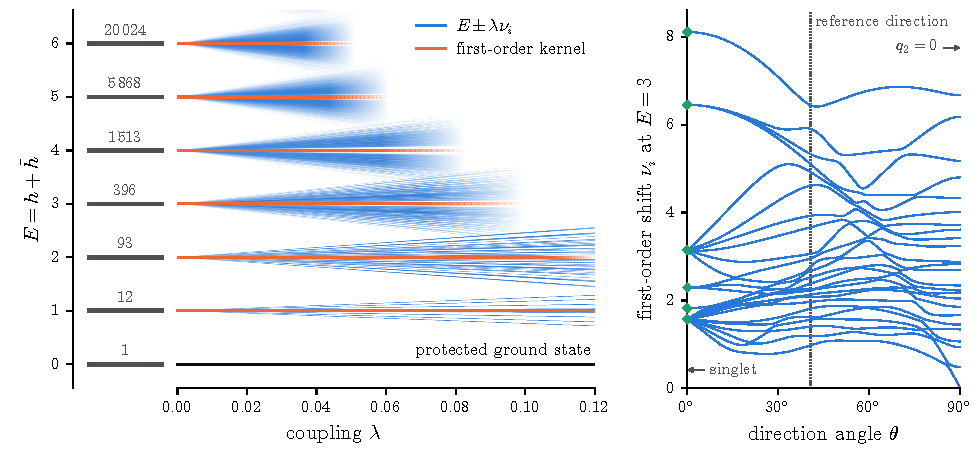
\includegraphics[width=.75\textwidth]{fig_spectrum_direction.pdf}
\caption{The scalar spectrum near the Kummer point.
{\it Left:} At $\lam=0$ the massive primaries of the invariant sector form exactly degenerate blocks at integer $E$ above the protected Ramond ground state (numbers: degeneracies). At first order each block splits into a band $E\pm\lam\nu_i$, while the states with vanishing first-order shift remain degenerate at $E$ (orange).
{\it Right:} Direction dependence in the space of deformations (exact at first order). The $25$ non-zero first-order shifts $\nu_i$ of one fully resolved $E=3$ sub-block, plotted along the great circle $q(\theta)\in S^3$ from the singlet $q_{\rm s}=(0,0,-1,0)$ (green diamonds) through the reference direction (dotted) to the triplet ``mirror'' $q_2=0$.}
\label{fig:spectrum}
\end{figure*}

The K3 sigma model is an $\mathcal N=(4,4)$ superconformal field theory with central charge $c=6$. Its moduli space is the $80$-dimensional Grassmannian $O(4,20)/O(4)\times O(20)$ up to discrete identifications \cite{Seiberg:1999xz,Aspinwall:1996mn,Nahm:1999ps}. At special points in moduli space the model is relatively well understood: at its orbifold points the theory is a free orbifold of a torus model, and at its Gepner points it is rational \cite{Gepner:1987vz,Gepner:1987qi}. The elliptic genus and the $\frac12$-BPS ground states are protected \cite{Dijkgraaf:1996xw,Eguchi:2010ej,Eguchi:1987wf}, while additional $\frac14$-BPS states at special points can lift \cite{Keller:2019suk}. In the D1-D5 system, the $\frac14$-BPS states that survive the deformation have recently been characterized \cite{Benjamin:2021zkn,Chang:2025rqy,Bintanja:2026uwk}, and chaos has even been investigated within the BPS sector itself, where the states are exactly degenerate and chaos must be detected by means other than level statistics \cite{Chen:2024oqv,Chen:2026vml,Belin:2026vfd}. In contrast, our focus will be on the non-BPS spectrum: away from the solvable points very little is known about the non-BPS states beyond perturbation theory (see however \cite{Afkhami-Jeddi:2021qkf,Keller:2023ssv}). We simply ask: \emph{are the non-BPS scaling dimensions Wigner-Dyson distributed as we deform away from a solvable point?} The natural data to analyze is the spectrum of primaries at fixed spin, which removes the obvious spectral correlations due to Virasoro symmetry and modular $T$-invariance. Any additional symmetries have to be resolved as well, since symmetries superpose statistically independent spectra and dilute their correlations \cite{Guhr:1997ve}.

The mechanism we use was identified in \cite{Srdinsek:2020bpq} for the double sine-Gordon model: the exactly degenerate spectrum of the free theory is lifted at first order in perturbation theory by a matrix whose eigenvalue spacings are Wigner-Dyson distributed when the two cosines are mixed with comparable coefficients, crossing over to Poisson statistics near the integrable limits. At first order the overall coupling only rescales this matrix, so the statistics depend only on the mixing. In that model the perturbations are relevant, so the deformed theory is a massive QFT and the first-order levels are finite-volume energies. We realize the same mechanism with an exactly marginal deformation, along which the theory remains conformal, so that the first-order splitting is a spectrum of anomalous dimensions of two-dimensional CFTs.

The same mechanism can be observed in perturbative anomalous dimensions \cite{McLoughlin:2020zew,McLoughlin:2022jyt,Baume:2026jyt} (see also \cite{Caputa:2026hvh}), in the matrices of second-order anomalous dimensions of $\frac14$-BPS states of the deformed symmetric orbifold of $\Tf$ at finite $N$ \cite{Zhang:2026jnf,Gaberdiel:2026jor}, and in spin systems with highly degenerate spectra \cite{Abdelshafy:2025ddx}. By contrast, in the planar limit of the symmetric orbifold the singlet and triplet perturbations admit an asymptotic integrable description \cite{Gaberdiel:2023lco,Frolov:2023pjw,Gaberdiel:2025smz} (see however \cite{Fabri:2025rok}), while the second-order shifts at fixed energy are close to Poisson \cite{Zhang:2026jnf}.\footnote{The planar limit suppresses the mixing of different cycle structures that leads to level repulsion at finite $N$. The Kummer model is closely related to $N=2$.}

At the Kummer point of the square torus at the free-fermion radius, the scalar states in the symmetry sector studied below form highly degenerate blocks at integer energies. The first-order splitting of each degenerate block by an exactly marginal deformation is then given by a finite matrix that can be computed using only free-field data. Figure~\ref{fig:spectrum} shows the spectrum and its deformation for the first six blocks. The moduli that blow up the $16$ fixed points symmetrically span a four-dimensional space of exactly marginal deformations, whose directions form a three-sphere of unit quaternions. Along a {\it generic} direction in this space, we find that the first-order shifts in fully resolved symmetry sectors exhibit GOE spectral statistics. Genericity is essential: we identify special directions on the three-sphere (among them the singlet deformation studied throughout the D1-D5 literature), which lead to deformations with enhanced symmetry either of the spectral sector we study or of the full theory.


\section{The K3 model and the space of deformations}
\label{sec:theory}

\paragraph*{The Kummer point.}
We start from the free $c=6$, $\mathcal N=(4,4)$ theory of four real bosons $X_{A\dot A}$ (the coordinates of a square torus $\Tf$), plus four left- and four right-moving real fermions $\psi^{\alpha A}$ and $\bar\psi^{\dot\alpha A}$, in the conventions of \cite{Guo:2019ady} (see also \cite{Avery:2010er}). The indices $A,\dot A$ are spinor indices of the $SU(2)_1\times SU(2)_2$ rotations of the tangent space of $\Tf$, an ``internal'' symmetry of the free fields that is broken by the lattice of the torus. Similarly, $\alpha,\dot\alpha$ are spinor indices of the two R-symmetries, $SU(2)_L\times SU(2)_R$. We work in the Ramond sector, in units $\alpha'=2$, with all four circles at the free-fermion radius $R=2$, where each compact boson is equivalent to a free Dirac fermion \cite{Ginsparg:1988ui}. The Fock states are labeled by their left- and right-moving momenta and integer oscillator levels (Supplemental Material (SM)~\cite{SupplementalMaterial}, Sec.~\ref{SM-app:kummer}); weights are measured relative to the Ramond ground state energy $\frac{c}{24}=\frac14$.

The Kummer orbifold gauges the reflection $(X,\psi,\bar\psi)\to-(X,\psi,\bar\psi)$ and gives the K3 sigma model at an orbifold point of its moduli space \cite{Dijkgraaf:1996xw,Seiberg:1999xz}. Its untwisted sector consists of the reflection-even states. In addition, each of the $16$ fixed points $x=\pi R\,\bff$, $\bff\in\{0,1\}^4$, carries a twisted sector in which all fields are antiperiodic. The ground state energies of the twisted bosons and fermions cancel, and the twisted states have the weights:
\begin{equation}
\label{eq:weights_tw}
h=N^{\rm tw}_L\,,\qquad \bar h=N^{\rm tw}_R\,,\qquad N^{\rm tw}_{L,R}\in\tfrac12\mathbb Z_{\ge0}\,,
\end{equation}
with $N^{\rm tw}_L+N^{\rm tw}_R\in\mathbb Z$ imposed by the orbifold projection (SM Sec.~\ref{SM-app:kummer}). 

Below, we will evaluate matrix elements of twist deformations of the Kummer model. To this end, it is useful to note that the model is closely related to the symmetric orbifold $\Sym^2(\Tf)$ \cite{Lunin:2001pw,Avery:2010er,Guo:2019ady} and to employ the associated covering space methods. The correspondence and momentum conventions are reviewed in SM Sec.~\ref{SM-app:firstorder}.\\

\paragraph*{Symmetry sectors.}
The half-period translations $U_\bt\colon  x\mapsto x+\pi R\,\bt$, $\bt\in\{0,1\}^4$, commute with the reflection and form a $\mathbb Z_2^4$ symmetry of the orbifold \cite{Taormina:2011rr,Gaberdiel:2013psa}, which is preserved by the deformations considered below. We label its $16$ eigenspaces, the symmetry sectors, by $\bs\in\{0,1\}^4$:
\begin{equation}
 {\cal H}_\bs = \big\{ |\Psi\rangle\colon \;\; U_\bt |\Psi \rangle = (-1)^{\bs \cdot \bt} |\Psi \rangle  \text{ for all } \bt \big\}\,.
\end{equation}
Such a sector contains the untwisted states whose momentum quantum numbers are congruent to $\bs$ modulo $2$ and one copy of the twisted tower \eqref{eq:weights_tw}, built by acting with oscillator modes on the combination $\frac14\sum_\bff(-1)^{\bs\cdot\bff}|\bff\rangle$ of the twisted ground states.\footnote{Note that $U_\bt |\bff\rangle = |\bff+\bt\rangle$, so $\frac14\sum_\bff(-1)^{\bs\cdot\bff}|\bff\rangle$ diagonalizes $U_{\bt}$.} At spin zero, the untwisted energies of a sector $\bs$ lie on $\mathbb Z+\frac14|\bs|$, where the weight $|\bs|$ is the number of non-zero components of $\bs$, while the twisted energies are integers. Since the deformation introduced below is built on a twist field, it only connects untwisted and twisted states, so that first-order mixing can only occur in the invariant sector $\bs=0$ and at the odd levels of the sector of weight $|\bs|=4$ (SM Sec.~\ref{SM-app:kummer}). We focus on the invariant sector.

In the invariant sector, reversing the right-moving fields alone, $(\bar\partial X,\bar\psi)\to-(\bar\partial X,\bar\psi)$, is a further involution, which is a symmetry of this sector only (SM Sec.~\ref{SM-app:kummer}). The deformations discussed below preserve it and we refer to it as $Z_R$.\\

\paragraph*{The marginal deformations.}
For each fixed point $\bff$, the corresponding twisted sector contains an NS-NS chiral primary $\twist_\bff^{++}$ of weights $h=\bar h = \frac12$ and R-charges $J_0^3 = \bar{J}_0^3=\frac12$. Acting on it with the supercurrents $G^\alpha_{\dot A}=\psi^{\alpha A}\partial X_{A\dot A}$ and $\bar G^{\dot\alpha}_{\dot A}=\bar\psi^{\dot\alpha A}\bar\partial X_{A\dot A}$, we generate the superdescendants $G^{-}_{\dot A,-\frac12}\bar G^{-}_{\dot B,-\frac12} \twist_{\bff}^{++}$. These have weights $h=\bar h=1$ and generate four real exactly marginal deformations associated with $\bff$, often called blow-up modes \cite{Dixon:1986qv,Nahm:1999ps}. We consider the four translation-invariant combinations of
these deformations, with equal coefficients at all fixed points:
\begin{equation}
\label{eq:Dc}
\Dc=\frac{1}{2\sqrt2}\,\cMat^{\dot A\dot B}\,G^{-}_{\dot A,-\frac12}\bar G^{-}_{\dot B,-\frac12}\twist^{++} \; + \; \text{h.c.}\,,
\end{equation}
where $\twist^{++}=\frac14\sum_\bff\twist^{++}_\bff$.
The Hamiltonian on the circle is deformed at first order:
\begin{equation}
\label{eq:HDc}
H(\lam)=H_0+\lam\,\Dcz \,,\quad\;\; \Dcz=\int_0^{2\pi}d\sigma\,\Dc(\sigma,0)\,.
\end{equation}
Each $\Dc$ is the top component of a short multiplet and hence an exactly marginal deformation that preserves conformality and $\mathcal N=(4,4)$ supersymmetry. Hermiticity of $\Dc$ implies that only the combination $\frac{1}{2}(\cMat+\epsilon \cMat^* \epsilon^T)$ contributes to the coefficient matrix. We can therefore take $\cMat^{\dot A \dot B}$ to be a real quaternion:
\begin{equation}
\label{eq:quaternion}
\cMat=q_0 \, \mathds{1}+ i \,(q_1\sigma_x+q_2\sigma_y+q_3\sigma_z)\,,\qquad q\in\mathbb R^4\,.
\end{equation}
The normalization $\langle\Dc(z)\Dc(0)\rangle=|q|^2/|z|^4$ fixes $|q|=1$, so the directions of deformation form a three-sphere $q\in S^3$. The unit $q=(0,0,-1,0)$, for which $\cMat^{\dot A\dot B}=\epsilon^{\dot A\dot B}$, is the $SU(2)_2$-invariant singlet deformation that is standard in the D1-D5 literature \cite{Avery:2010er,Guo:2019ady}. The other three units span the triplet of \cite{Gaberdiel:2025smz} (see also \cite{Keller:2019suk} and SM Sec.~\ref{SM-app:deformations}).\\

\paragraph*{States.}
We restrict to the Ramond-Ramond sector (the other sectors follow by spectral flow). For each copy of a massive representation of the two $\mathcal N=4$ algebras, we keep the superconformal primary with $J^3_0=\bar J^3_0=-\frac12$. In a massive representation this is the lowest weight of the R-spin-$\frac12$ doublet \cite{Eguchi:1987wf}. We consider scalar primaries, $h=\bar h$, and denote by $E=h+\bar h\ge0$ the energy above the Ramond-Ramond ground state. At $E=0$ the only state with these properties is the protected Ramond vacuum, the lowest weight of the R-spin-$(\frac12,\frac12)$ ground states. At the undeformed orbifold point, the selected primaries at each integer energy $E>0$ span a highly degenerate subspace $\B(E)$, which we call a {\it block} (see Fig.~\ref{fig:spectrum} for the first six block sizes).\\

\paragraph*{Symmetry resolution.}
The deformation \eqref{eq:HDc} preserves the two $\mathcal N=4$ algebras and breaks the additional continuous internal symmetries of the orbifold point (see SM Sec.~\ref{SM-app:symmetries}). Having removed the superconformal multiplet degeneracies by our choice of primaries, we now need to resolve the remaining discrete symmetries within each block ${\cal B}(E)$.

Discrete symmetries organize the space of directions $q\in S^3$. The point group of the square torus, worldsheet parity $\cMat\mapsto \cMat^T$, $\cMat\mapsto-\cMat$ and, on the invariant sector, a rotation of the right-movers alone all relate different directions with identical spectra in the invariant sector. They act on $S^3$ as reflections in $16$ mirrors, i.e., the great two-spheres $q_\mu=0$ and $q_\mu=\pm q_\nu$ with $\mu\neq\nu$ (End Matter). On a mirror, the corresponding reflection becomes an additional symmetry, which is reflected in the level statistics.

The singlet lies at a locus where nine mirrors meet, and the triplet spans the mirror $q_2=0$. Figure~\ref{fig:spectrum} (right) shows the effect on the first-order shifts of one sub-block along a great circle from the singlet through the reference direction to the mirror $q_2=0$: at the singlet the 25 shifts are highly degenerate, and away from it they split and repel. 

Away from the mirrors, the point-group transformations that leave $\cMat$ unchanged form the stabilizer $\Hc$. On the scalar primaries considered here, its action reduces to two commuting $\mathbb Z_2$ symmetries, whose eigenvalue signs label the four one-dimensional characters of $\Hc$ (the trivial character has both signs positive). The commuting involution $Z_R$ provides a third sign, giving eight possible sub-blocks at each level. Since all twisted scalar states at level $E$ have $Z_R=(-1)^E$, the four sub-blocks with $Z_R=-(-1)^E$ contain only untwisted states, which do not mix at first order and stay at $E$. At the even levels there is one further, hidden $\mathbb Z_2$, which we found numerically (End Matter). We present most of our numerics for a reference direction on $S^3$, drawn at random, which lies far from every mirror ($5.5^\circ$ from the nearest one):
\begin{equation}
\label{eq:qgen}
q_{\rm ref}=(-0.318,\ 0.096,\ -0.760,\ 0.559)\,.
\end{equation}


\section{First-order degenerate perturbation theory}
\label{sec:firstorder}

\begin{figure*}[t]
\centering
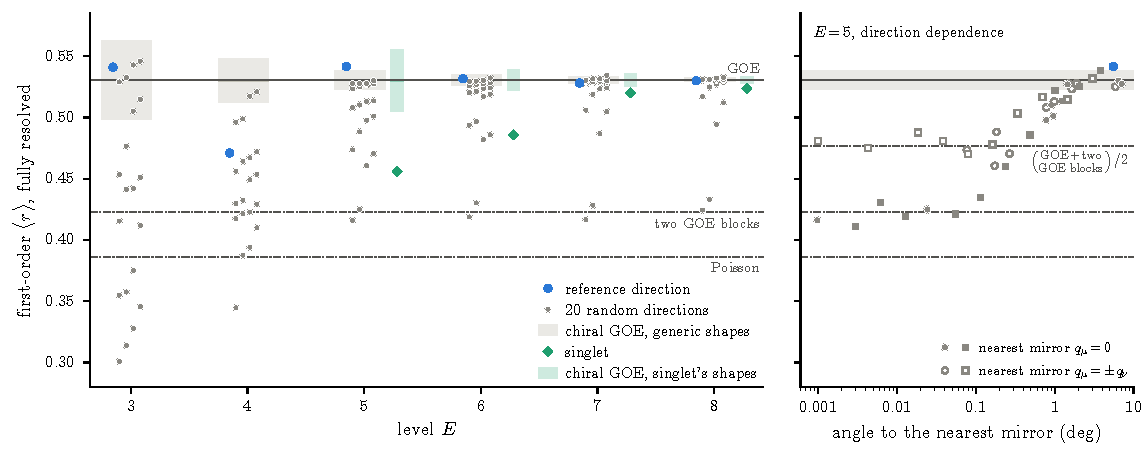
\includegraphics[width=\textwidth]{fig_firstorder_vs_E_sample.pdf}
\caption{{\it Left:} Symmetry-resolved first-order gap ratio along the reference direction (blue), along $20$ further directions drawn at random (gray), and along the singlet direction (green). Gray and green bands show the mean and standard deviation of $\rmean$ for chiral GOE matrices with shapes matched to the numbers of twisted states and distinct positive singular values. The singlet points resolve the singlet's own symmetries, including the hidden $\mathbb Z_2$ at the even levels. {\it Right:} $\rmean$ at $E=5$ for the reference direction plus the same $20$ random directions (circles) and $20$ further directions close to a single mirror (squares). We show the dependence of $\rmean$ on the angle $\delta$ to the nearest mirror, which illustrates the signatures of split sub-blocks in the vicinity of different types of mirrors ($\delta\to 0$).}
\label{fig:firstorderE}
\end{figure*}

\paragraph*{The first-order matrix.}
Let $\{|\Psi_a\rangle\}_{a=1}^{d_E}$ be an orthonormal basis of the degenerate block $\B(E)$. The first-order energy shifts are $\lam$ times the eigenvalues of $\langle\Psi_b|\Dcz|\Psi_a\rangle$. The level-preserving part of $\Dcz$ commutes with both $\mathcal N=4$ algebras, so the problem closes on superconformal primaries. Further, since the deformation contains a twist field, it only couples the $d_+$ untwisted states to the $d_-$ twisted states, with $d_E=d_++d_-$. In the basis of untwisted followed by twisted states, the first-order matrix is
\begin{equation}
\label{eq:Mc}
\HB^{(1)}=\begin{pmatrix}0&\Mc^{\dagger}\\ \Mc&0\end{pmatrix}\,.
\end{equation}
The $d_-\times d_+$ matrix $\Mc$ is constructed from free-field chiral twist amplitudes, as explained in End Matter. If $\nu_i$ are its non-zero singular values, the levels split as $E\pm\lam\nu_i$, while $d_++d_--2\rank\Mc$ states remain at $E$.\\

\paragraph*{Exact structures in the perturbed spectrum.}
The orbifold quantum $\mathbb Z_2$, $\mathcal Q$, acts as $+1$ on untwisted and $-1$ on twisted states \cite{Gaberdiel:2013psa}. It anticommutes with $\Dcz$, giving the paired shifts $\pm\nu_i$. The $Z_R$ selection rule above bounds the rank of $\Mc$ by the number of untwisted states with $Z_R=(-1)^E$ (End Matter), so that roughly half of the states of each level remain at $E$ at first order. In all generic cases we checked, the non-zero singular values are distinct; the statistics below concern these values.\\

\paragraph*{Gap ratios.}
For a generic direction a fully resolved sub-block is one of the four characters of $\Hc$ with $Z_R=(-1)^E$, split further by the hidden $\mathbb Z_2$ at the even levels. In each of them we sort the distinct singular values, $\nu_1<\dots<\nu_n$, and form the gap ratios:
\begin{equation}
\label{eq:r}
r_i=\frac{\min(\delta\nu_i,\delta\nu_{i+1})}{\max(\delta\nu_i,\delta\nu_{i+1})}\,,\qquad \delta\nu_i=\nu_{i+1}-\nu_i\,.
\end{equation}
We then combine (``pool'') the ratios of all sub-blocks of a level into a single sample and compute their mean $\rmean$ \cite{Oganesyan:2007wpd,Atas:2013gvn}. Its reference values are $0.5307$ for the GOE, $0.5996$ for the Gaussian unitary ensemble (GUE), $0.3863$ for Poisson statistics, and $0.423$ for a superposition of two independent GOE spectra of equal size, the signature of an unresolved $\mathbb Z_2$ \cite{Giraud:2020mmb}. We compare with the chiral GOE (class BDI in the Altland-Zirnbauer classification \cite{Verbaarschot:1994qf,Altland:1997zz}; see End Matter), i.e., matrices of the form \eqref{eq:Mc} with $\Mc$ replaced by a real Gaussian random matrix of the same shape.\\

\paragraph*{Results.}
In Fig.~\ref{fig:firstorderE} we show the gap ratios for the reference direction and other random directions, as well as for the singlet (see the table in End Matter for the underlying data). At every level except $E=4$ the reference direction agrees with the GOE value to within $1.4\,\sigma$ (for $E=4$, where the deficit is common to all directions, see End Matter). Resolving every symmetry, including the hidden $\mathbb{Z}_2$, is essential: at $E=6$, before the hidden $\mathbb Z_2$ is resolved, the reference direction gives $\rmean_{\rm ref}=0.509$, well below the GOE value. At $E=8$, the sub-block transforming trivially under the stabilizer gives $\rmean_{\rm ref}=0.434$ before this $\mathbb Z_2$ is resolved, and $0.536$ and $0.531$ in its two resolved eigenspaces (End Matter).

The right panel of Fig.~\ref{fig:firstorderE} shows a sample of random directions for $E=5$: directions that lie farther from the mirrors agree better with GOE statistics. Closer to a mirror, the additional symmetries are only weakly broken, which washes out the RMT statistics.  On a mirror $q_\mu=0$ these symmetries exactly split every sub-block, giving the value of two independent spectra, while on a mirror $q_\mu=\pm q_\nu$ they map two characters of $\Hc$ onto each other and split the others. As the level spacing decreases with $E$, the distance from a mirror required to break its symmetry also shrinks.

The singlet direction is fixed by the whole point group, and the hidden $\mathbb Z_2$ splits several of its sub-blocks at the even levels (End Matter). Even fully resolved, its gap ratio lies below the GOE value at every level, well below at $E=5,6$ and by about two standard deviations at $E=7,8$. Unlike a generic direction, it also features exact degeneracies within its resolved sub-blocks; e.g., at $E=8$, $583$ out of $10721$ non-zero values repeat, most of them at a single value $\nu=\pi$.\\

\paragraph*{Wigner surmise and number variance.}
The gap ratio tests the correlation of neighboring levels without reference to the mean level density. To test correlations over many levels we unfold each sub-block separately with a smooth fit of its counting function $N(\nu)$, the number of levels not larger than $\nu$, and then compute the distribution $P(s)$ of the unfolded nearest-neighbor spacings and the number variance $\Sigma^2(L)$, i.e., the variance of the number of unfolded levels in an interval of length $L$ (see SM Sec.~\ref{SM-app:firstorder}). Figure~\ref{fig:spacings} shows that at $E=8$ the spacing distribution follows the GOE Wigner surmise $P(s)=\frac{\pi s}{2}e^{-\pi s^2/4}$ over the sampled range, and that the number variance follows the GOE prediction \cite{Mehta2004} up to $L=10$ at $E=7,8$. At $E=6$ it rises above the GOE curve for $L\gtrsim4$, but the sub-blocks of this level are too small for a reliable separation of the fluctuations from the mean level density (SM Sec.~\ref{SM-app:firstorder}).

We again contrast with the unfolded spectrum of the singlet deformation, which matches the GOE surmise less well for nearest-neighbor spacings and deviates significantly from the GOE in the number variance (Fig.~\ref{fig:spacings}). The reason is that the singlet's first-order levels cluster at special values: neighboring levels still repel, which keeps its gap ratio relatively close to the GOE value at $E=7,8$, but the spectrum lacks long-range rigidity.

\ifdefined\arXivversion
  \begin{figure*}[t] %
  \centering
  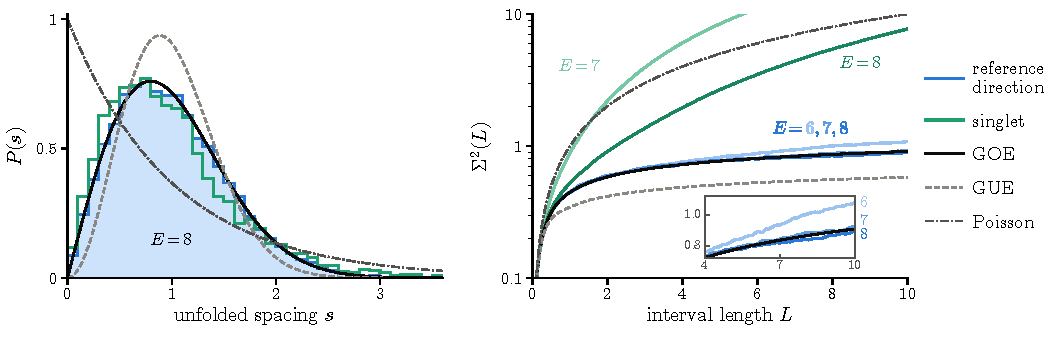
\includegraphics[width=.85\textwidth]{fig_spacings_singlet_twocol.pdf}
\else
  \begin{figure}[b] %
  \centering
  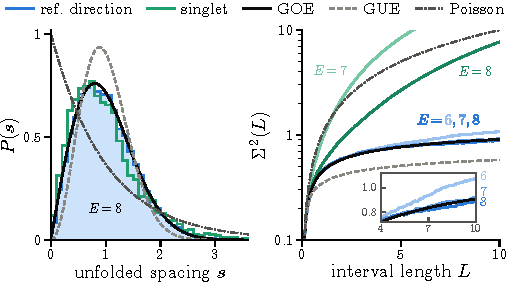
\includegraphics[width=\columnwidth]{fig_spacings_singlet_onecol.pdf}
\fi
\caption{Unfolded first-order spectra along the reference direction (blue) and the singlet (green). {\it Left:} Distribution of the nearest-neighbor spacings at $E=8$, compared with Wigner surmises and the Poisson distribution.
{\it Right:} The number variance measuring long-range correlations.}
\label{fig:spacings}
\ifdefined\arXivversion\end{figure*}\else\end{figure}\fi


\section{Conclusions}
\label{sec:conclusion}

We have shown that, deformed away from the Kummer orbifold along a generic direction, the K3 sigma model has primaries whose leading anomalous dimensions exhibit the level statistics of the GOE. The statistics are computed from the first-order matrices of an exactly marginal deformation inside the degenerate blocks of the free orbifold. As standard degenerate perturbation theory dictates, these matrices are computed from free-field data, so the statement holds for the deformed theory as $\lam\to0^+$. At finite coupling it holds only while the second-order shifts stay small compared to the first-order spacings.\footnote{Random matrix level statistics at weak coupling does not by itself imply ergodicity (cf.\ \cite{Abdelshafy:2025ddx}): $H_0$ is conserved to this order, and different levels remain uncorrelated.} The result requires a generic direction on the quaternion sphere of $\mathbb Z_2^4$-symmetric blow-up moduli and the resolution of every exact symmetry. Special directions, among them the well-known singlet deformation, carry additional symmetries or extra structures that wash out random matrix statistics. We identified the hidden $\mathbb Z_2$ only numerically and it would be interesting to understand its origin.

Our analysis is restricted to the invariant sector $\bs=0$. The odd levels of the sector of weight $|\bs|=4$ provide a separate first-order problem, while the remaining $14$ sectors are split only at second order. Using the relation to the symmetric orbifold $\Sym^2(\Tf)$, it would be interesting to follow the first-order statistics in $\Sym^N(\Tf)$ as $N$ grows, where the planar second-order shifts are close to Poisson \cite{Zhang:2026jnf,Gaberdiel:2026jor}, and to connect the onset of random matrix statistics at infinitesimal coupling with the random matrix universality expected for holographic CFTs. It would also be interesting to relate the random matrix statistics of the non-BPS spectrum found here to the proposed diagnostics of BPS chaos \cite{Chen:2024oqv,Chen:2026vml,Belin:2026vfd}.


Beyond first order the spectrum can be computed using an energy truncation $E\le\Lam$, renormalized in the manner of Hamiltonian truncation \cite{Hogervorst:2014rta,Rychkov:2014eea,Elias-Miro:2017xxf}: at second order, the counterterms that remove its cutoff dependence follow from the operator product of the perturbation with itself. The analysis of the truncation and the second-order primary spectrum will be presented elsewhere \cite{toappear}. Exact marginality suggests a second route: at every coupling the deformed theory is again a CFT, so the level dynamics becomes a flow of the conformal data along the conformal manifold \cite{Pechukas:1983,Yukawa:1985zz}, which can in principle be integrated \cite{Behan:2017mwi}. As the coupling grows, the first-order bands of neighboring levels touch and their spectra merge. It is worth investigating whether random matrix statistics then extend across levels, and to look for other signatures of chaos, such as eigenstate thermalization \cite{Deutsch:1991msp,Srednicki:1994mfb,Lashkari:2016vgj}.\\


\paragraph*{Acknowledgments.}
We thank A.\ Dei and I.\ Zadeh for discussions and comments. FMH is supported by UK Research and Innovation (UKRI) under the UK government's Horizon Europe funding Guarantee EP/X030334/1. MR is supported by an NSERC Discovery Grant and used the clusters of the Digital Research Alliance of Canada for the numerical computations. AI tools (Claude Opus and Fable, ChatGPT Pro for Academic Researchers) were used for the numerical implementation and plots, for some analytic calculations and for refining ideas.

\paragraph*{Data availability.}
The code and data that support the findings of this Letter are openly available~\cite{HaehlRozali:2026code}.

\nocite{Larsen:1999uk,Keller:2011xi,Hartman:2014oaa,Gava:2002xb,Gaberdiel:2015uca,Keller:2019yrr,Guo:2020gxm}
\bibliographystyle{apsrev}
\bibliography{references}


\appendix
\section*{End Matter}
\setcounter{equation}{0}
\renewcommand{\theequation}{A\arabic{equation}}


\paragraph*{Matrix elements and rank bound.}
The states of a degenerate block $\B(E)$ are linear combinations of two kinds of Fock states (SM Sec.~\ref{SM-app:kummer}): twisted states $|t\rangle=|t^Lt^R\rangle$ are products of chiral oscillator states on the invariant twisted ground state, while untwisted states $|u\rangle$ are reflection-even combinations of products $|u^Lu^R\rangle$. The spatial integral over the deformation operator conserves the spin, and between spin-zero states at the same level it gives $\langle\Psi_b|\Dcz|\Psi_a\rangle=2\pi\langle\Psi_b|\Dc(0,0)|\Psi_a\rangle$. Finally, the level-preserving part of $\Dcz$ maps primaries to primaries because it commutes with the two $\mathcal N=4$ algebras (SM Sec.~\ref{SM-app:firstorder}).

Between products of chiral states, the local matrix elements factorize:
\begin{equation}
\label{eq:factor}
\begin{aligned}
&\big\langle t_b\big|G^{-}_{\dot A,-\frac12}
 \bar G^{-}_{\dot B,-\frac12}\twist^{++}
 \big|u_a\big\rangle=\langle t_b^L|{\cal A}_{\dot A}|u_a^L\rangle
         \langle t_b^R|{\cal A}_{\dot B}|u_a^R\rangle\,.
\end{aligned}
\end{equation}
Matrix elements between reflection-even or symmetry-adapted states follow by linearity. The chiral twist maps ${\cal A}_{\dot A}$ are computed with the covering space method of the symmetric orbifold following \cite{Lunin:2001pw,Avery:2010er,Guo:2019ady}. Only their level-preserving parts enter above. With the momentum-lattice and orbifold restrictions understood, the rectangular matrix in the first-order Hamiltonian \eqref{eq:Mc} is
\begin{equation}
\label{eq:Mc-chiral}
\Mc=\sqrt2\,\pi\,\cMat^{\dot A\dot B}
{\cal A}_{\dot A}\otimes{\cal A}_{\dot B}\,.
\end{equation}
At each level, the chiral maps are finite matrices and the construction is algorithmic.

The grading by $\mathcal Q$ guarantees at least $|d_+-d_-|$ zero modes. A stronger bound follows from $Z_R$. At level $E$, $Z_R$ reverses every right-moving mode, so that all twisted scalar states have $Z_R=(-1)^{2\bar h}=(-1)^E$ and only untwisted states with this eigenvalue can mix with them. If their number is $\tilde d_+$, then
\begin{equation}
\label{eq:rankbound}
\rank(\Mc)\le\tilde d_+\,.
\end{equation}
At odd levels, $Z_R$ pairs the untwisted momentum orbits without fixed points, so $\tilde d_+=d_+/2$ (SM Sec.~\ref{SM-app:kummer}). At even levels its two eigenspaces need not have equal dimensions, and we compute $\tilde d_+$ directly. Along a generic direction the bound is saturated at $E=3,5,7$; at $E=4,6,8$ saturation fails by $1$, $84$, $57$ states, respectively. Thus the odd-level zero-mode count is as small as allowed by the grading and the rank bound. The total number of unshifted states is $d_++d_--2\rank\Mc$.\\


\paragraph*{Symmetry resolution.}
The point group of the square torus ($192$ orientation-preserving signed permutations of the coordinates), worldsheet parity $\cMat\mapsto \cMat^T$, and $\cMat\mapsto-\cMat$ relate equivalent deformed theories. Their action forms a reflection group whose ten mirrors are the intersections of $S^3$ with the hyperplanes $q_2=0$, $q_\mu=0$ and $q_\mu=\pm q_{\nu\neq\mu}$ with $\mu,\nu\in\{0,1,3\}$. Each mirror is a great two-sphere on which the corresponding reflection becomes an additional symmetry of the deformed theory. The invariant sector has one further equivalence: a rotation of the right-movers alone, which maps the deformation along $\cMat$ onto that along $\cMat\,i\sigma_x$, $\cMat\,i\sigma_y$ or $\cMat\,i\sigma_z$, so that their invariant-sector spectra coincide exactly (SM Sec.~\ref{SM-app:symmetries}). This adds the six mirrors $q_2=\pm q_\mu$, on which the corresponding reflection is an additional symmetry of the invariant sector. The $16$ mirrors cut $S^3$ into $384$ spherical tetrahedra, and no two directions in the same tetrahedron are related by the above discrete maps.\\

The symmetries we can easily identify along a generic direction, i.e., the stabilizer $\Hc$ and $Z_R$, are not enough to resolve every sub-block. For even levels, the gap ratio of the sub-block of the trivial character of $\Hc$ with $Z_R=+1$ is that of two superposed spectra, the signature of an unresolved symmetry~\cite{Giraud:2020mmb}. 

An exact symmetry commutes with $H_0$ and with $\Dcz$, including its matrix elements between different levels, which first-order perturbation theory does not use. The first-order matrix of one level is therefore not enough to identify such a symmetry, since operators built from its own singular vectors commute with it as well. In practice, we thus look numerically for subspaces that $H_0$ and $\Dcz$ leave jointly invariant, using the matrices projected onto the selected primaries through $E=6$, including off-level matrix elements up to $E=6$ together with the matrix elements of $\Dcz$ between different levels. A symmetry commuting with both acts within each level and would be diagonal in the eigenbasis of $H(\lambda)=H_0+\lambda\Dcz$ for every $\lambda$. Therefore, eigenvectors computed at two different couplings (we choose $\lambda=0.2$ and $0.35$) are orthogonal when they lie in different eigenspaces of the symmetry, while those in the same eigenspace generically overlap. The eigenspaces can thus be found by computing all eigenvectors at each of the two couplings and linking an eigenvector at one coupling to one at the other whenever their overlap exceeds a small threshold. The connected components of the resulting graph are the eigenspaces. 

\begin{figure}[t]
\centering
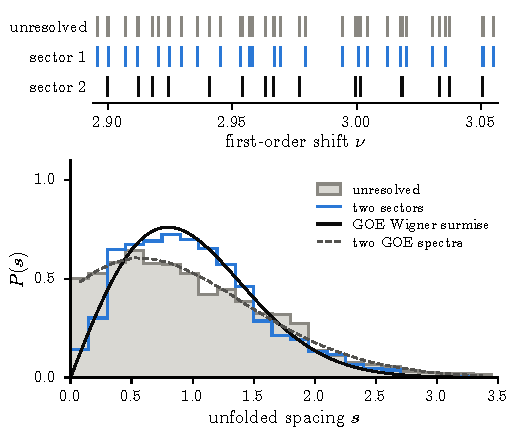
\includegraphics[width=\columnwidth]{fig_hiddenZ2.pdf}
\caption{The hidden $\mathbb Z_2$ along the reference direction for $E=6$, in the sub-block of the trivial character of $\Hc$ with $Z_R=+1$: a total of $1350$ first-order values split into eigenspaces of $899$ and $451$ values. {\it Top:} $40$ consecutive levels of the unresolved sub-block and the same levels split into the two eigenspaces of the $\mathbb Z_2$. {\it Bottom:} Distribution of the unfolded nearest-neighbor spacings for the unresolved sub-block (gray) and for its two eigenspaces (blue), compared with the GOE Wigner surmise and two independent GOE spectra superposed in the proportion $899:451$ (dashed).}
\label{fig:hiddenZ2}
\end{figure}

An unresolved symmetry superposes two independent spectra, whose levels do not repel each other. Figure~\ref{fig:hiddenZ2} shows this for the reference direction at $E=6$: in the $40$ levels at the top, levels that come very close almost always lie in different eigenspaces. The distribution of unfolded spacings (bottom) shows the same: for the unresolved sub-block, $P(s)$ stays finite as $s\to0$, like that of two independent GOE spectra superposed in the proportion $899:451$, whereas within each eigenspace the levels repel as in the GOE. The gap ratio confirms this: the unresolved sub-block has $\rmean_{\rm ref}=0.432$, close to the value $0.441\pm0.009$ of the two superposed GOE spectra. Its two eigenspaces give $0.524$ and $0.519$, respectively. Pooled with the three other sub-blocks of this level, they give the value $\rmean_{\rm ref} = 0.532$ reported in Sec.~\ref{sec:firstorder}. At $E=8$ we proceed differently. Since the involution does not depend on the direction (see below), it commutes with the first-order matrix of every direction, and the overlap test above can be applied to the singular vectors of $\Mc$ at two generic directions. At $E=4$ and $6$ this reproduces the eigenspaces found from the truncated Hamiltonian. At $E=8$ it splits the $9216$ values of the sub-block into eigenspaces of $6137$ and $3079$ values, with $\rmean_{\rm ref}=0.536$ and $0.531$.\\

The same $\mathbb Z_2$ acts along the singlet direction. The involution that splits the sub-block does not depend on the direction: it commutes with $\Dcz$ for every $\cMat$ and with the whole point group, but it is not an element of the point group. Along the singlet, whose larger symmetry group divides the states into smaller sub-blocks, it splits several of those with $Z_R=+1$ at the even levels, again with eigenspaces in a ratio of about two to one. It mixes oscillator states with momentum states of the same energy. Left unresolved, it lowers the singlet’s gap ratio from $0.486$ to $0.465$ at $E=6$ and from $0.524$ to $0.494$ at $E=8$.\\


\paragraph*{Statistical analysis.}
The chiral GOE is the expected symmetry class: CPT composed with the R-symmetry Weyl reflections defines an antiunitary symmetry $T$ with $T^2=+1$ that preserves each fully resolved sub-block along a generic direction. Its first-order matrix therefore admits a real symmetric representation (SM Sec.~\ref{SM-app:symmetries}). Moreover, the twisted states outnumber the untwisted states that couple to them by a factor of about two, so that the relevant matrices are far from square: the smallest singular value lies far from the hard edge at zero, and the bulk statistics are that of the GOE.

The following table gives the untwisted and twisted dimensions $d_\pm$, the rank of $\Mc$, the gap ratio for the reference direction (pooling fully resolved sub-blocks), and the standard deviation $\sigma$ of the mean gap ratio for a single chiral GOE spectrum of matrices with the same sizes:
\begin{equation*}
\begin{tabular}{cccccc}
\toprule
$E$ & $d_+$ & $d_-$ & $\rank \Mc$ & $\rmean_{\rm ref}$ & $\sigma$ \\
\midrule
3 & 200    & 196   & 100    & $0.541$ & $0.032$ \\
4 & 729    & 784   & 304   & $0.471$ & $0.018$ \\
5 & 2952   & 2916  & 1476  & $0.542$ & $0.0081$ \\
6 & 10420  & 9604  & 5448  & $0.532$ & $0.0042$ \\
7 & 28288  & 28224 & 14144 & $0.528$ & $0.0026$ \\
8 & \;76881\; & \;79524\; & \;36840\; & $ \;0.530\; $ & $\;0.0016\;$ \\
\bottomrule
\end{tabular}
\end{equation*}
To compute $\sigma$, we pool the gap ratios for $3000$ independent realizations, each containing one real Gaussian matrix per sub-block, with as many rows as twisted states and as many columns as distinct non-zero singular values. At $E=8$ the two-direction method does not determine how the twisted states divide between the two eigenspaces of the hidden $\mathbb Z_2$. We divide them in proportion to the sizes of the eigenspaces, and $\sigma$ does not depend on this choice at the quoted accuracy. We observe a significant deviation from the GOE expectation at $E=4$, which is a property of this level and not of the reference direction: over $3000$ random directions more than $4^\circ$ from every mirror, the pooled gap ratio is $0.495$ on average. In the three sub-blocks without a hidden $\mathbb Z_2$, the deficit comes from the upper end of the spectrum: the ten gap ratios at the top of each sub-block average $0.40$ and the remaining ones $0.53$. There the highest level is isolated and the two levels below it are nearly degenerate. Along the singlet direction the same sub-blocks have a nondegenerate top level and an eightfold degenerate one below it, which splits into two levels and three pairs at first order in the distance from the singlet. We found no comparable structure at $E=3,5,6$ and no further exact symmetry in these sub-blocks. The two eigenspaces of the hidden $\mathbb Z_2$ give $\rmean=0.45$ each.


\ifdefined\arXivversion
  \clearpage
  \onecolumngrid
  \SMsetup
  \input{\SMfilename}
\fi


\end{document}
